\section{Provable Security Analysis of Privacy}
\label{sec:privacy}


In this section, we will give the proof that UPPRESSO is defensive to both IdP-based login tracing and RP-based identity linkage, based on DDH assumption\cite{GoldwasserK16}, the computational problem. 


\noindent\textbf{DDH Assumption.}
$\mathbb{G}$ is a n-order  cyclic additive group of $E(\mathbb{F}_q)$, where $q$ and $n$ are large primitive number, and $P$ is the generator of $\mathbb{G}$.  For any probabilistic polynomial time (PPT) algorithm $D$, the distributions, \{$P$, $aP$, $bP$, $abP$\}$_{a,b \in \mathbb{Z}_n}$ and \{$P$, $aP$, $bP$, $cP$\}$_{a,b,c \in \mathbb{Z}_n}$, are computationally indistinguishable. There is a negligible $\sigma(k)$, where $k$ is the security parameter. 
\begin{multline*}
    \ \ \ \ \ \ \ Pr[D(P, aP, bP, abP)=1]\\-Pr[D(P, aP, bP, cP)=1]=\sigma(k)\ \ \ \ \ \ \ \ 
\end{multline*}

\noindent\textbf{IdP-based identity linkage.} 
It can be found in figure~\ref{fig:process} that $PID_{RP}$ is the only data related with RP's identity accessible to IdP. Moreover, $PID_{RP}$ is created based on $ID_{RP}$ and the IdP uncontrolled random number $N_U$. As $N_U$ is randomly chosen in $\mathbb{Z}_n$,  $PID_{RP}$ can be also seemed  randomly chosen in $\mathbb{G}$ to IdP. Therefore, obviously IdP cannot trace the user's login RPs, so that IdP-based identity linkage is not possible in UPPRESSO.

\noindent\textbf{RP-based identity linkage.} 

\begin{figure}[t]
  \centering
  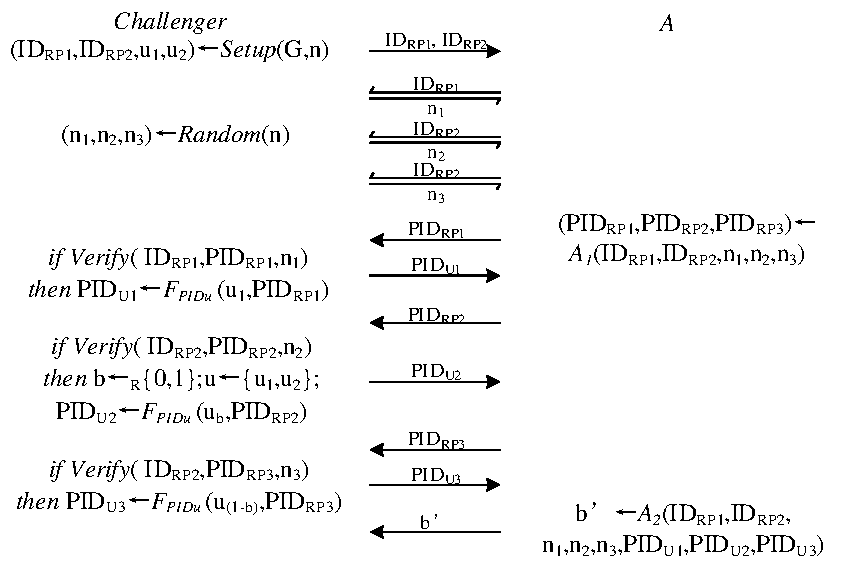
\includegraphics[width=1\linewidth]{fig/game0.pdf}
  \caption{Game 0.}
  \label{fig:game0}
\end{figure}
In the \emph{RP-based identity linkage} scenario, collusive RPs conduct the malicious behavior against IdP and users to relate the user in different RPs. It can be considered as a $Game$ guessing whether $PID_U$s for different RPs belong to the same user.  In this $Game$ IdP and users act as the challenger, and RPs act as the adversary. 

\textbf{If only the adversary cannot take any advantage on guessing whether $PID_U$s belong to same user, RP-based identity linkage is considered impossible in UPPRESSO.}


Following, we are going to build the model of Game to show how the adversary interactive with the challenger. Here we describe the challenger's actions in the Game.
\begin{itemize}
\item[-] Initialization: In the initialization phase, the challenger generates the $ID_{RP}$s and $ID_U$s for multiple RPs and users, based on the initialization algorithm $Setup(G,n)$ where $G$ and $n$ have been already defined in table~\ref{tbl:notations}.
\item[-] Random number generation: While challenger receives the $ID_{RP}$s from adversary, it generates random numbers $N_U \in \mathbb{Z}_n$ for each $ID_{RP}$s creating $PID_{RP}$ using algorithm $Random(n)$.
\item[-] $PID_U$ generation: In this phase, challenger firstly receives and  verifies whether $PID_{RP}$ is correctly generated based on $ID_{RP}$ and corresponding $n$ (i.e., the algorithm $Verify(ID_{RP},PID_{RP},N_U)$). Then it generates the $PID_U$ using the algorithm $F_{PID_U}(ID_U,PID_{RP})$ and sends it to adversary.
\end{itemize}

Firstly we give the realistic model of the $ID_U$-guessing Game, shown as figure~\ref{fig:game0}. In this Game, adversary firstly achieves 2 $IR_{RP}$s and 3 $N_U$s and generates 3 $PID_{RP}$s. In the challenger's view, these $PID_{RP}$s are related with 3 $N_U$s respectively. Following the challenger generates $PID_U$s for different $PID_{RP}$s based on the 2 $ID_U$s generated in initialization phase. 
Then challenger generates the random $b$=0 or 1. $PID_{U1}$ is generated based on $ID_{U1}$. However $PID_{U2}$ and $PID_{U3}$ are generated according to $b$. That is, $PID_{U2}=ID_{Ub}PID_{RP2}$, and $PID_{U3}=ID_{U(1-b)}PID_{RP3}$  

Finally adversary returns the $b'$. While $b=b'$ is true, we consider the adversary succeeds, that means the RP-identity-linkage is possible in UPPRESSO.
We define the event [$b'=b$] in Game 0 as $\Gamma$. The probability $Pr[\Gamma]$ must be 1/2 as if the adversary cannot take any advantage of guessing $b$ (i.e.  whether $PID_U$s belong to same $ID_U$). Therefore, it is proved that UPPRESSO is protected from RP-based identity linkage only if $Pr[\Gamma]=1/2$.

Then we build the ideal model of Game, of which the probability  that an adversary succeeds to guessing $b$ is 1/2. The model is shown as figure~\ref{fig:game1}. We use $z$ and $r$ for generating $PID_{U2}$ and $PID_{U3}$ instead of $ID_{U1}$ and $ID_{U2}$. As $z$ and $r$ is randomly generated and unknown to $A$, the adversary has no information about $b$. We  define the event [$b'=b$] in Game 1 as $\Gamma_1$. $Pr[\Gamma_1]$ must be equal to 1/2. 

Therefore, we only need to prove that $|Pr[\Gamma_1]-Pr[\Gamma]|=\sigma(n)$, where $\sigma(n)$ is negligible. Here we give another model of Game, shown as figure~\ref{fig:game2}. We can find that in fact it only sets the exact values of the parameters defined in Game 0, such as $ID_{RP2}=xID_{RP1}$, $u_1=y$ and $u_2=r$(r is a random number).  Here we define the event [$b'=b$] in Game 2 as $\Gamma_2$. There should be $Pr[\Gamma_2]=Pr[\Gamma]$.

We are going to prove that $|Pr[\Gamma_1]-Pr[\Gamma_2]|=\sigma(n)$. In each Games, adversary derives the $b'$ from collected data, $\{ID_{RP1},ID_{RP2},n_1,n_2,n_3,PID_{U1},PID_{U2},PID_{U3}\}$, with the algorithm $A_2$. Now we replace the parameters in Game 1 and Game 2 with exact values. In Game 1, $b'_{game1}\gets A_2(P,xP,n_1,n_2,n_3,yn_1P,zP,rP)$, and in Game 2, $b'_{game2}\gets A_2(P,xP,n_1,n_2,n_3,yn_1P,xyn_2P,rn_3P)$ or $b'_{game2}\gets A_2(P,xP,n_1,n_2,n_3,yn_1P,rn_2P,xyn_3P)$. 
However, $n_1$, $n_2$, $n_3$ are randomly chosen unrelated with $ID_U$ by challenger and able to be eliminated by adversary. Therefore, there is, in Game 1, $b'_{game1}\gets A_2(P,xP,yP,zP,rP)$, and in Game 2, $b'_{game2}\gets A_2(P,xP,yP,xyP,xrP)$. As $r$ is randomly chosen and unknown to adversary, both $rP$ and $xrP$ are random points and cannot bring any extra advantage for adversary to guessing $b$.  The final procedure is $b'_{game1}\gets A_2(P,xP,yP,zP)$ and $b'_{game2}\gets A_2(P,xP,yP,xyP)$. Therefore, there must be no non-negligible difference value between the success probability in Game 1 and Game 2 according to DDH assumption. Otherwise, we can build the PPT distinguishing algorithm breaking DDH assumption based on the adversary. 

\noindent\textbf{Distinguishing algorithm.} The distinguishing algorithm $D$ is shown as figure~\ref{fig:dalgorithm}. 
The inputs of the algorithm is $\{P,X,Y,Z\}$. While the input is in the form $\{P,xP,yP,zP\}_{x,y,z \in \mathbb{Z}_n}$, for the adversary it is the Game 1. As the input is $\{P,xP,yP,xyP\}_{x,y \in \mathbb{Z}_n}$, for the adversary it is the Game 2. So, there is,
\begin{equation*}
   Pr[D(P,xP,yP,zP)=1]=Pr[{\Gamma_1}]
\end{equation*}
\begin{equation*}
   Pr[D(P,xP,yP,xyP)=1]=Pr[{\Gamma_2}]
\end{equation*}

Therefore, $|Pr[\Gamma_1]-Pr[\Gamma_2]|=\sigma(n)$, where $\sigma(n)$ is negligible, and $n$ is the security parameter. So, the adversary has no advantage to guessing $b$ in Game 0, that means he cannot distinguish whether two $PID_U$s for different RPs belong to the same user or not. 

The RP-based identity linkage attack is not possible in UPPRESSO.


\begin{figure}[t]
  \centering
  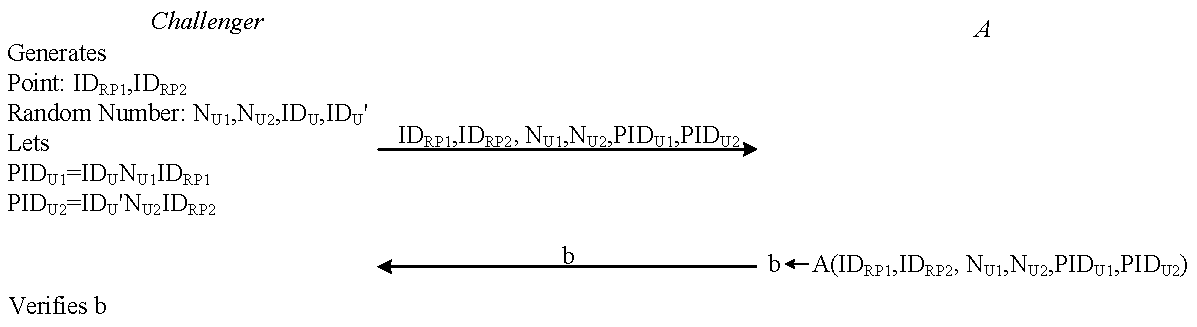
\includegraphics[width=1\linewidth]{fig/game1.pdf}
  \caption{Game 1.}
  \label{fig:game1}
\end{figure}




\begin{figure}[t]
  \centering
  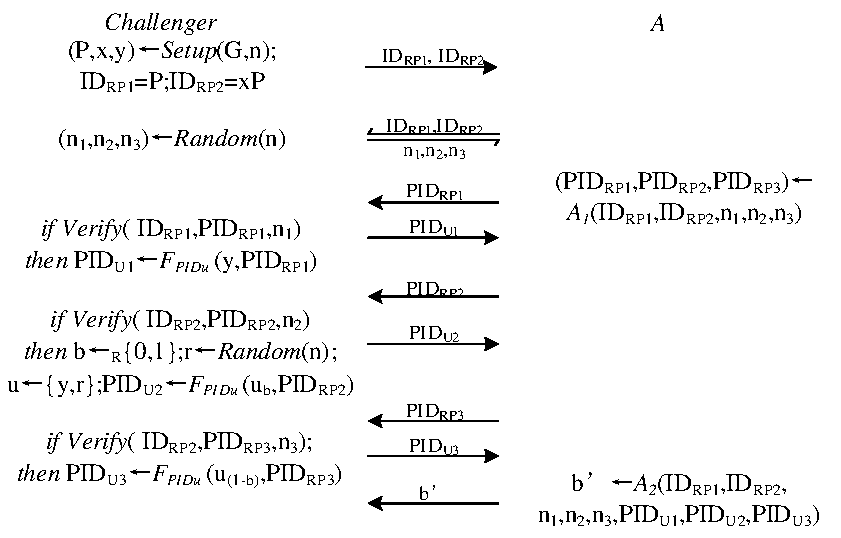
\includegraphics[width=1\linewidth]{fig/game2.pdf}
  \caption{Game 2.}
  \label{fig:game2}
\end{figure}

\begin{figure}[t]
  \centering
  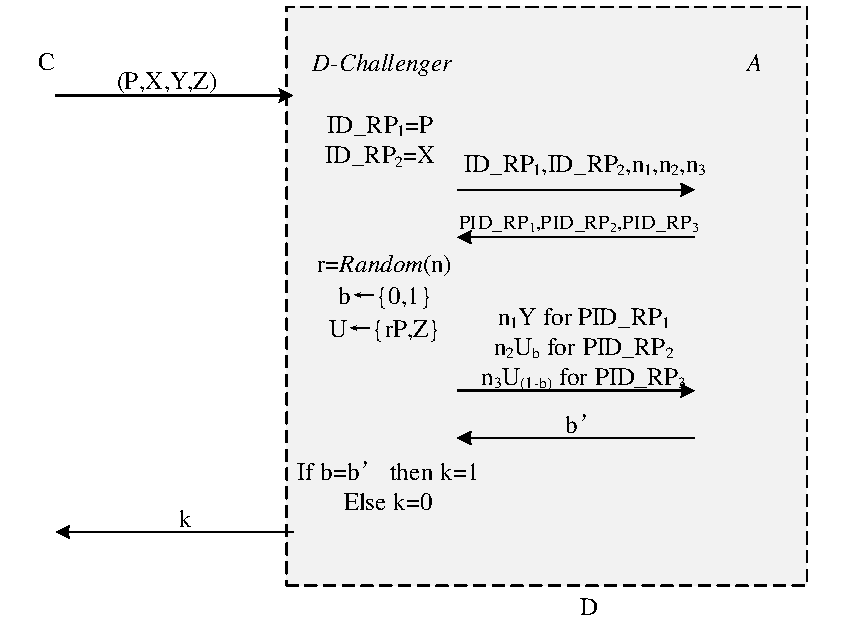
\includegraphics[width=1\linewidth]{fig/dalgorithm.pdf}
  \caption{Distinguishing algorithm.}
  \label{fig:dalgorithm}
\end{figure}